\documentclass[a4paper,
fontsize=11pt,
%headings=small,
oneside,
numbers=noperiodatend,
parskip=half-,
bibliography=totoc,
final
]{scrartcl}

\usepackage[babel]{csquotes}
\usepackage{synttree}
\usepackage{graphicx}
\setkeys{Gin}{width=.6\textwidth} %default pics size

\graphicspath{{./plots/}}
\usepackage[ngerman]{babel}
\usepackage[T1]{fontenc}
%\usepackage{amsmath}
\usepackage[utf8x]{inputenc}
\usepackage [hyphens]{url}
\usepackage{booktabs} 
\usepackage[left=2.4cm,right=2.4cm,top=2.3cm,bottom=2cm,includeheadfoot]{geometry}
\usepackage{eurosym}
\usepackage{multirow}
\usepackage[ngerman]{varioref}
\setcapindent{1em}
\renewcommand{\labelitemi}{--}
\usepackage{paralist}
\usepackage{pdfpages}
\usepackage{lscape}
\usepackage{float}
\usepackage{acronym}
\usepackage{eurosym}
\usepackage{longtable,lscape}
\usepackage{mathpazo}
\usepackage[normalem]{ulem} %emphasize weiterhin kursiv
\usepackage[flushmargin,ragged]{footmisc} % left align footnote
\usepackage{ccicons} 
\setcapindent{0pt} % no indentation in captions

%%%% fancy LIBREAS URL color 
\usepackage{xcolor}
\definecolor{libreas}{RGB}{112,0,0}

\usepackage{listings}

\urlstyle{same}  % don't use monospace font for urls

\usepackage[fleqn]{amsmath}

%adjust fontsize for part

\usepackage{sectsty}
\partfont{\large}

%Das BibTeX-Zeichen mit \BibTeX setzen:
\def\symbol#1{\char #1\relax}
\def\bsl{{\tt\symbol{'134}}}
\def\BibTeX{{\rm B\kern-.05em{\sc i\kern-.025em b}\kern-.08em
    T\kern-.1667em\lower.7ex\hbox{E}\kern-.125emX}}

\usepackage{fancyhdr}
\fancyhf{}
\pagestyle{fancyplain}
\fancyhead[R]{\thepage}

% make sure bookmarks are created eventough sections are not numbered!
% uncommend if sections are numbered (bookmarks created by default)
\makeatletter
\renewcommand\@seccntformat[1]{}
\makeatother

% typo setup
\clubpenalty = 10000
\widowpenalty = 10000
\displaywidowpenalty = 10000

\usepackage{hyperxmp}
\usepackage[colorlinks, linkcolor=black,citecolor=black, urlcolor=libreas,
breaklinks= true,bookmarks=true,bookmarksopen=true]{hyperref}
\usepackage{breakurl}

%meta
%meta

\fancyhead[L]{B. Kaden\\ %author
LIBREAS. Library Ideas, 36 (2019). % journal, issue, volume.
\href{http://nbn-resolving.de/}
{}} % urn 
% recommended use
%\href{http://nbn-resolving.de/}{\color{black}{urn:nbn:de...}}
\fancyhead[R]{\thepage} %page number
\fancyfoot[L] {\ccLogo \ccAttribution\ \href{https://creativecommons.org/licenses/by/4.0/}{\color{black}Creative Commons BY 4.0}}  %licence
\fancyfoot[R] {ISSN: 1860-7950}

\title{\LARGE{Zu unserem Titelbild. Die Normalität eines Kernreaktors}}
\author{Ben Kaden} % author

\setcounter{page}{1}

\hypersetup{%
      pdftitle={Zu unserem Titelbild. Die Normalität eines Kernreaktors},
      pdfauthor={Ben Kaden},
      pdfcopyright={CC BY 4.0 International},
      pdfsubject={LIBREAS. Library Ideas, 36 (2019).},
      pdfkeywords={Forschungszentrum Jülich},
      pdflicenseurl={https://creativecommons.org/licenses/by/4.0/},
      pdfcontacturl={http://libreas.eu},
      baseurl={http://libreas.eu},
      pdflang={de},
      pdfmetalang={de}
     }



\date{}
\begin{document}

\maketitle
\thispagestyle{fancyplain} 

%abstracts

%body
\begin{figure}[h!]
\centering
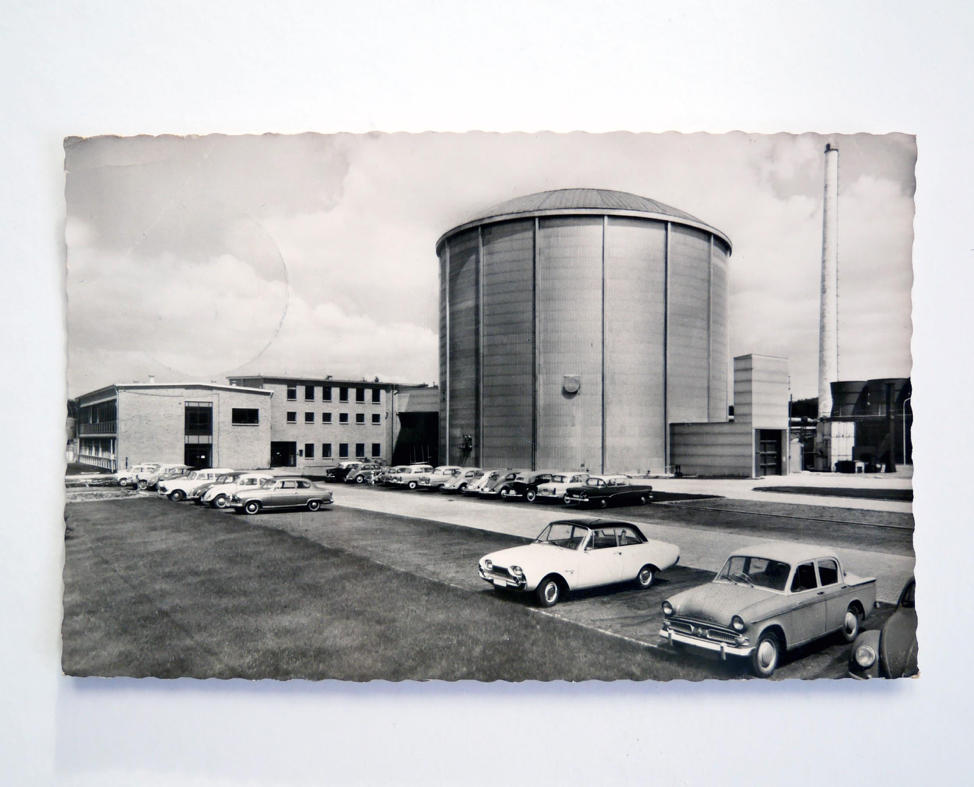
\includegraphics{cover.png}
\caption{Titelbild der Ausgabe 36}
\end{figure}

\hypertarget{i}{%
\subsubsection{I}\label{i}}

Das Kernforschungszentrum Jülich war wahrlich kein Selbstläufer. In den
fortschreitenden 1950er Jahren hatte man beschlossen, die vom Zweiten
Weltkrieg schwer zerstörte und sich eher mühsam wiederfindende Stadt im
Westen Nordrhein-Westfalens zum Standort eines Kernforschungszentrums
werden zu lassen.

\enquote{Wir stehen vor dieser dunklen Wand, hinter der sich eines der
kostbarsten Geschenke verbirgt, das die Natur für den Menschen bereit
hält: die Atomenergie.} So wird der frühe Rundfunkexperte,
Ingenieurwissenschaftler, Sozialdemokrat und später zuständige
Staatssekretär Leo Brandt aus einem Appell an die Lokalpolitiker
zitiert.\footnote{o.A.: Lästige Konkurrenz. In: Der SPIEGEL, 01.01.1958,
  S. 18f. \url{https://www.spiegel.de/spiegel/print/d-41760318.html}} Es
galt an das Atomzeitalter anzuklopfen. Und in Deutschland antwortete man
auf das Versprechen der Zukunft fast traditionell eher verhalten. Auch
Leo Brandt, der zuvor als Verkehrsverwalter maßgeblich auf die
Elektrifizierung der Bundesbahn hingearbeitet hatte, wusste das:
\enquote{In Deutschland ist die Frage, ob diese Energieform überhaupt
von Nutzen ist, leider sehr umstritten.} In Düren zum Beispiel. Dort war
er gescheitert, kurioserweise, aus heutiger Sicht, am Widerstand der
Braunkohlelobby..

Die fehlende Innovationsbereitschaft seiner Landsleute und der daraus
resultierende Rückstand im Bereich des technisch-wissenschaftlichen
Fortschritts hatten Leo Brandt schon bei seiner Tätigkeit für die
Wehrmacht beschäftigt. Trotz eifrigem Bemühens, den
Entwicklungsvorsprung der britischen Radartechnik vor der deutschen
irgendwie aufzuholen, scheiterten er und seine Arbeitsgruppe und er
betreute ab 1946 den Fuhrpark der Stadtwerke in Düsseldorf. In recht
kurzer Zeit zum Staatssekretär aufgestiegen wurde, fand er sich also
1957 an einer energiepolitischen Forschungsfront. Es gelang ihm
tatsächlich die Kernforschungsanlage Jülich des Landes
Nordrhein-Westfalen (KFA) durchzusetzen.

Leo Brandts Enthusiasmus kam freilich bei den Energieversorgern seiner
Zeit und seines Bundeslands kaum an. RWE beispielsweise zeigte sich sehr
uninspiriert. Heinrich Schöller, Technikvorstand des Unternehmens,
sprach sich in der frisch gegründeten Fachzeitschrift \emph{Die
Atom-Wirtschaft} dafür aus, abzuwarten, wie sich diese bislang kaum
erprobte Technologie überhaupt ersteinmal entwickeln würde, bevor große
Ressourcen investiert werden:

\enquote{In die auch im Ausland noch in den Anfängen stehende technische
Großanwendung der Atomenergie brauchen wir dann nicht mit unreifen und
unwirtschaftlichen großen Projekten einzutreten. Wir vermeiden dadurch
die Verschwendung von Milliardenbeträgen.}\footnote{Zitiert nach ebd.}
Die wurden freilich woanders, nämlich in Großbritannien investiert. Dort
förderte man die Atomenergie in den späten 1950ern mit umgerechnet 11
Milliarden Mark, in Deutschland waren es dagegen nur etwa 58
Millionen.\footnote{ebd.}

Diskursgeschichte wiederholt sich offenbar recht gern. Denn die
Pro-Atomenergie-Stimmen begegneten dem Argument möglicherweise
fehlgehender Großinvestitionen mit dem Verweis auf eher anders gelagerte
Bedenken, nämlich um die damals noch sehr enge Verschränkung von
Kohlebergbau und Energiewirtschaft. Diese Lobby bremse den Weg in die
Zukunft, die von unglaublicher Energienachfrage gekennzeichnet sein wird
unddie allein durch Atomkraft bedient werden kann - so in etwa die
eingedampfte Argumentationslinie.

Die Zurückhaltung bei politischen Akteuren und Energieunternehmen
änderte sich nach und nach auch dank intensiver und argumentativ
ausgefeilter Pro-Atom-Lobbyarbeit, denn den Anschluss an die Zukunft und
vor allem auch an staatliche Investitionen in diese Zukunft wollte man
nicht verlieren. Für die Gesellschaft wurde Kernenergie zum Versprechen
hochstilisiert und entwickelte sich später zum Gegenstand eines
harmlosen Weihnachtssketches von Loriot. Jülich wurde zu einem Ort der
Zukunftserwartung inszeniert. Hier sollten die Lösungen für den
unabsehbaren, in jedem Fall aber riesigen Energiebedarf in einem
postfossilen Zeitalter gefunden werden. Die kleine Stadt wurde so zu
einem Standort der Spitzenforschung mit entsprechendem internationalen
Publikum.

\hypertarget{ii}{%
\subsubsection{II}\label{ii}}

Auch Ansichtskarten selbst lassen sich als eine einstige
Zukunftstechnologie mit heute kaum mehr nachvollziehbarem
wirtschaftlichen Potential sehen. Mit dem Aufkommen des Mediums in den
1870er Jahren entstand ein ungeahnte hyperaktive Nutzung mit utopischer
Aufladung. Zunächst als Korrespondenzkarte in Anlehnung und zur
Ergänzung des Mediums Brief eingeführt, führte die Einführung einer
Bildseite zu einer Entfesselung des Mediums.

Begleitet vom Ausbau und der Standardisierung des Postwesens, verbunden
mit einer Ökonomisierung, die die Kommunikationskosten für die Einzelnen
senkte und eben der damals noch nicht selbstverständlichen
Verbildlichung der Welt rückte diese enger und vielfältiger zueinander.
Die Weltausstellungen wurden folgerichtig zum Multiplikator. Die
Leistungsschau der Nationen wurde auf Souvenirkarten zum Mitnehmen und
besser noch verschickten umfänglich dokumentiert. Wo gerade keine
Weltausstellung stattfand, fand man leicht andere Gründe und Motive für
das kuriose neue Medium, das schnell auch zum Wirtschaftsfaktor wurde.
Souvenirkarten erlebten einen Boom und damit verbunden auch eine Kritik,
wie wir sie heute von Instagram kennen. In gewisser Weise erfüllten sie
eine ganz ähnliche Funktion.

Die zweite Nutzungsphase setzte mit der Jahrhundertwende ein. Dank einer
\enquote{divided back} genannten formalen Innovation wurden sie zu einem
tatsächlichen Kommunikationsmedium für geschriebene Nachrichten. Statt
zuvor bestenfalls mit einer Handvoll Wörter ein Souvenir zu
personalisieren, war es nun möglich, 200, 300 Zeichen, manchmal auch
mehr zu verschicken. Ansichtskarten wurden zu einem twitteresken
Direct-Messaging-Dienst, immer potentiell halböffentlich und
entsprechend oft auch spielerisch gebraucht. Wo sich mehr sagen ließ,
vervielfältigten sich auch die kommunikativen Gebrauchsweisen. Man
begann nun Nachrichten tatsächlich auch reziprok auszutauschen. Halbwegs
erschwinglich, verlässlich und flexibel wurde die Postkarte zu einem
Medium der Alltags- und auch kommerzieller Koordination. Sie diente zum
Bestellen, zum Ankündigen und Absagen von Besuchen und zur Übermittlung
von Fernschachzügen.

Die Mengen waren enorm. Um 1900 transportierte das britische Postsystem
419 Millionen Postkarten.\footnote{Für weitere Ausführungen zum Thema
  siehe auch: Ben Kaden: So, dass soll es gewesen sein. Viele liebe
  Grüsse. Ein kurzer Blick auf die Ansichtskartenkultur der DDR. In:
  Christoph Liepach: Gera ostmodern. Leipzig: Sphere publishers, 2019.
  S. 18-31} Die Zahl sollte sich schnell stetig vervielfachen, bis ein
externes Ereignis, nämlich der Erste Weltkrieg, die Dynamik aus dem
Geschehen nahm. Das lag auch daran, dass ein Großteil der Ansichtskarten
weltweit deutscher Herkunft waren. Etwas verzögert gestartet, war
Deutschland auf diesem Feld, wenn man so will, Exportweltmeister und
lieferte um 1907 allein in die USA etwa 700-800 Millionen
Karten.\footnote{Vgl. Jeffrey L. Meikle: Postcard America. Austin:
  University of Texas Press, 2016, S.15} Diese Versorgung endete abrupt
aufgrund von Strafzöllen auf deutsche Produkte. Parallel wurden, als
letzte und düstere Blüte zum Abschluss des ersten goldenen Zeitalters
des Mediums, Postkarten im Ersten Weltkrieg aufgrund ihrer
niedrigschwelligen Nutzbarkeit zu einem zentralen Feldpostmedium. Von
den Heimatfronten kamen nicht selten Propagandamotive und
Durchhalteappelle und aus den Schützengräben, sofern noch möglich,
Lebenszeichen.

Die zweite Blütezeit setzte wenige Jahre später ein. Das Medium
Ansichtskarte verschwand nämlich keinesfalls wie die einstmals führenden
deutschen Postkartenhersteller, sondern wurde zum normalen und
omnipräsenten Teil der kommunikativen Alltagskultur. Die Vorteile -
flexibel, informell, schnell und preiswert - blieben. Die Bildseite
stand mal mehr, gern aber auch weniger im Vordergrund des konkreten
Gebrauchs. Bilder tauchten mittlerweile ebenfalls in höherer Qualität in
Magazinen und Zeitschriften auf und sättigten auch dort einen
entsprechenden Appetit. Die Ansichtskarte war nicht mehr die
bombastische Innovation, sondern eher eine im Kleinen, massiv
angetrieben durch Fortschritte im Bereich der Fotografie, Drucktechnik
und Gestaltung sowie, ausschlaggebend, durch die zunehmende Mobilität
der Menschen. Das Bild diente weniger dazu, ein Motiv zu zeigen. Sondern
dazu, zu zeigen, dass man sich selbst am dargestellten Ort befunden
hatte, vergleichbar mit dem zeitgenössischen Selfie-Tourismus Die
topographische Ansicht wurde zum Geotagging ihrer Zeit, die Sammlung zu
einer Kartei der Geografika.

So explodierte parallel zum Tourismus der Gebrauch der Ansichtskarten
ein weiteres Mal. Curt Teich, amerikanischer Ansichtskartentycoon mit
Wurzeln in Greiz, nutzte die Möglichkeiten des Offset-Drucks um für zwei
Jahrzehnte - circa 1930-1950 - den Markt in den USA zu dominieren. Von
ihm ist der Satz überliefert, das kein Ort zu klein sei, um nicht mit
Ansichtskarten repräsentiert zu werden.\footnote{Vgl. u.a. Monica Cure:
  Picturing the Postcard. Minneapolis, London: University of Minnesota
  Press, 2018. S. 198} Das Motto nahm man sich auch anderswo zu Herzen.
So strebte beispielsweise der Zentralverlag topographischer
Ansichtskarten der DDR, nämlich BILD UND HEIMAT Reichenbach (Vogtland),
offenbar eine nahezu repräsentative Vollabdeckung des Landes ab und dies
auch noch, als sich die Motivvielfalt in der alten Bundesrepublik längst
auf weitgehend tatsächlich touristische Inszenierungen konzentrierte.

\hypertarget{iii}{%
\subsubsection{III}\label{iii}}

In den 1960er Jahren traf nun die etwas ältere Innovation der
repräsentativen Ansichtskarte auf Jülich als Ort der
Zukunftstechnologie. Die Wissenschaftsmoderne, das Space Age, die
technologische und architektonische Reformulierung der Lebenswelt, die
Nachkriegsmoderne fanden im Medium Ansichtskarten eine niedrigschwellige
Ausdrucks- und Vermittlungsform. Die Errungenschaften der neuen Zeit,
fotografisch oft sehr anspruchsvoll in Szene gesetzt, waren nicht nur in
der um ihre Legitimität und Anerkennung ringenden DDR
ansichtskartentauglich, die jedem gelungenen Neubauviertel und Bau der
Ostmoderne ganze Serie widmete. Auch eine Parkstadt Bogenhausen wurde
eindrucksvoll auf diesem Medium inszeniert, allerdings nicht als
Schwarz-Weiß-Echt-Fotoabzug sondern in Agfacolor. Neueröffnete
Autobahnen und Stauseen ebenso. Industrieansichten finden sich, übrigens
auch aus der DDR, dagegen eher seltener.

Dennoch lässt sich für die Kernenergiebewegung in Westeuropa ein kleiner
Bestand an Aufnahmen mit recht typischen Bildmerkmalen identifizieren.
Teils wurde bereits die Bauphase mit dokumentiert, so zum Beispiel in
Philippsburg. In der Regel findet man aber Ansichten zu so klangvollen
Namen wie Biblis, Neckarwestheim, Würgassen-Beverungen, Forsmarks,
Zurzach und Leibstadt, die aus Vogelperspektive oder Fernsicht eine
menschengemachte Idealnatur (grün, blühend, geordnet) oft mit Flußlauf
zeigen und darin saubere, fast sterile Betonensemble teils skulpturaler
Qualität. Siedlungsstrukturen tauchen bestenfalls am Rand auf. Eine
bemerkenswerte Ausnahme bildet eine knallbunte Mehrbildkarte aus
Lingen/Ems mutmaßlich aus den 1980er Jahren. Sie zeigt das Kernkraftwerk
als normalen Stadtbestandteil neben Jugendherberge, Marktplatz und St.
Bonifatius Hospital. Nach der frühen Aufbau- und Betriebsphase und dem
Verlust der utopischen Kraft der Erzählung der Atomenergie, also bis
Anfang der 1980er weitgehend einer Normalisierung des Phänomens,
schwächte sich die Ansichtskartenpräsenz dieser Motivgruppe nach und
nach ab. Spätere Postkarten zum Thema stammen vorwiegend von kleinen und
größeren Kunstanstalten und Fotostudios sondern aus der
Öffentlichkeitsarbeit der Kraftwerksbetreiber selbst. Mit dabei: RWE.

Dass das Forschungszentrum Jülich auf einer Ansichtskarte gewürdigt
wurde, überrascht entsprechend nicht. Der Forschungsreaktor MERLIN zeigt
nicht nur eine frühe Wortspielfreude an Akronymen - \textbf{M}edium
\textbf{E}nergy \textbf{R}esearch \textbf{L}ight water moderated
\textbf{I}ndustrial \textbf{N}uclear reactor - sondern auch, dass die
Bundesrepublik nun in den frühen 1960er Jahren infrastrukturell zur
zeitgenössischen Großforschung und Technologieentwicklung aufgeschlossen
hat. Zumindest optisch. Alfred Böttcher, der wissenschaftlich-technische
Vorstand der Kernforschungsanlage, beklagte sich 1962 bitterlich: „Wir
haben noch nirgendwo Anschluß an das Ausland".\footnote{o.A.: Nicht
  einmal Geld für Kabel. Finanzielle Sorgen im Kernforschungszentrum
  Jülich. In:

  Nordwest Zeitung, 17.05.1962, S.16} MERLIN stand zwar und fuhr, wie
man sagte, bereits an. Aber die für die eigentlich geplanten Forschung
erforderlichen Anschlussinstitute waren weder vorhanden noch
ausfinanziert. Das wissenschaftliche Personal stand bereits wieder, so
Böttcher, vor dem Wechsel an besser funktionierende und bezahlende
Einrichtungen. Wie in unserem akuten Erinnerungsraum die
IT-Spezialist*innen, konnten sich die Kernphysiker*innen und
Radiolog*innen ihre Stellen in diesen Jahren und Arbeitsbedingungen
problemlos aussuchen. Aber wirklich sorgen musste sich Alfred Böttcher
nicht. Die Unternehmung war längst zu groß, als dass sie noch scheitern
durfte. Neben den großen Investitionssummen für die beiden
Forschungsreaktoren war das Forschungszentrum bereits zu diesem
Zeitpunkt ein maßgeblicher Strukturfaktor für die Region. Im Frühling
1963 arbeiten dort fast zweitausend Personen. Perspektivisch sollte sich
die Zahl mindestens verdreifachen. Dies führte naturgemäß zu einem
rapiden Zuwachs der Einwohnerzahl in Jülich und den umliegenden
Gemeinden.

Jülichs bekannteste Buchhandlung - Fischer, seit 2019 Thalia - entschied
sich vor dem Hintergrund der Medienpraxis dieser Jahre und der Bedeutung
des Forschungszentrums nachvollziehbar, die gezeigte Ansichtskarte mit
Blick auf Merlin aufzulegen. Durch die wohlgeordnete Inszenierung des
Mitarbeiterparkplatzes und des Reaktors, wird ein Ort der Arbeit
präsentiert und zwar angesichts des Modellmixes der geparkten
Automobile, ein ganz normaler, für Menschen von nebenan. Das Mittel- und
Bezugspunkt der Fotografie bildende Reaktorgebäude wirkt zwar hermetisch
und damit potentiell etwas geheimnisvoll, aber es überwältigt nicht.
Sympathisch dimensionierte Büro- und Begleitgebäude sowie der
Schornstein erzeugen eine Anschlussfähigkeit an die
Darstellungskonvention bekannter Produktionsinfrastrukturen. Das
Außergewöhnliche wird zugleich repräsentativ dargestellt, aber auch
normalisiert. Kein Aufbruch, eher stille und konzentrierte
Produktivität.

Die Kernforschungsanlage blieb freilich ähnlich wie die Atomenergie im
Prinzip in der Bundesrepublik immer umstritten. Die großen Erwartungen
erfüllten sich nicht, auch wenn der Reaktor auf Forschungs- und
Erkenntnisebene durchaus umfassend zum Wissensfortschritt der
einschlägigen Forschungsfelder führte. Der SPIEGEL schrieb 1981 in der
für seinen Stil üblichen blumigen Häme: \enquote{{[}D{]}ie
\enquote{Informationstagung} im Jülicher Kernforschungszentrum, der
Geburtsstätte des dabei gerühmten \enquote{Hochtemperaturreaktors}
(HTR), glich dann doch eher einer Versammlung von gutmeinenden Freunden
und Angehörigen am Bett eines Siechen.}

Sowie: \enquote{Nach 25 Jahren Entwicklungszeit und einem Einsatz von
mehr als zwei Milliarden Mark Steuergeldern aus Bonn und Düsseldorf (und
einigen Millionen Mark Industrie-Investitionen) lahmt das Projekt noch
immer.}\footnote{o.A.: Heiße Kugeln. In: Der SPIEGEL, 5/1981, S. 176-180}

Auch sonst arbeiteten diese und auch andere Publikationen gern die
Sumpfigkeit von Energiepolitik und Atomlobby dieser Jahre heraus. Dass
ausgerechnet am Standort Jülich ab den 1970ern das Potential für eine
Wende zu erneuerbaren Energien untersucht und als eher gering
eingeschätzt wurde, trug nicht unbedingt zur Vertrauensbildung bei.
Generell hatte Jülich wie auch die Kernenergie an sich aber durchgängig
mit der Akzeptanz von der Erzählung der saubersten und sichersten
Energieform zu kämpfen. Nach Tschernobyl waren im Prinzip außerhalb der
Lobby Hopfen und Malz verloren. Merlin war zu diesem Zeitpunkt schon gar
nicht mehr am Netz. Folgeskandale, wie die Häufung von Leukämie-Fällen
in Nähe der Anlage\footnote{o.A.: JÜLICH 12 Kinder an Leukämie erkrankt.
  In: Focus, 05.04.1993, S.11} ließen eventuelle Reste an Akzeptanz
weiter erodieren. Der schon Mitte der 1980er begonnene Abschied von der
Kernforschung und der Rückbau der Reaktoren kam entsprechend nahezu
folgerichtig und hielt noch lange manche negative Überraschung
bereit.\footnote{Frank Dohmen, Barbara Schmidt: Heißer Meiler. In:
  SPIEGEL online. 24.07.2009
  \url{https://www.spiegel.de/politik/deutschland/rueckbau-des-reaktors-juelich-heisser-meiler-a-637916.html}}
Das Forschungszentrum, längst ohne \emph{Kern-}, erfand sich erfolgreich
neu und forscht heute unter anderem zu erneuerbaren Energien\footnote{Siehe
  \url{https://www.fz-juelich.de/portal/DE/Forschung/_node.html}}. Auch
die dazugehörige Bibliothek ist renommiert und zeichnet sich unter
anderem durch einen starken Open Science-Bezug aus. Im September 2008
war MERLIN verschwunden. An seine Stelle pflanzte man, zurück zur Natur,
eine Eiche.

%autor
\begin{center}\rule{0.5\linewidth}{0.5pt}\end{center}

\textbf{Ben Kaden} ist Mitherausgeber der Zeitschrift LIBREAS. Library
Ideas

\end{document}
